\documentclass[12pt,letterpaper]{article}
\usepackage[utf8]{inputenc}
\usepackage[spanish]{babel}
\usepackage{graphicx}
\usepackage[left=2cm,right=2cm,top=2cm,bottom=2cm]{geometry}
\usepackage{graphicx} % figuras
% \usepackage{subfigure} % subfiguras
\usepackage{float} % para usar [H]
\usepackage{amsmath}
%\usepackage{txfonts}
\usepackage{stackrel} 
\usepackage{multirow}
\usepackage{enumerate} % enumerados
\renewcommand{\labelitemi}{$-$}
\renewcommand{\labelitemii}{$\cdot$}
% \author{}
% \title{Caratula}
\begin{document}

% Fancy Header and Footer
% \usepackage{fancyhdr}
% \pagestyle{fancy}
% \cfoot{}
% \rfoot{\thepage}
%

% \usepackage[hidelinks]{hyperref} % CREA HYPERVINCULOS EN INDICE

% \author{}
\title{Caratula}

\begin{titlepage}
\begin{center}
\large{UNIVERSIDAD PRIVADA-DE-TACNA}\\
\vspace*{-0.025in}
\begin{figure}[htb]
\begin{center}

\end{center}
\end{figure}
\begin{center}
    
\includegraphics[width=6cm, height=5cm]{img/upt.jpg}  
\end{center}

\vspace*{0.15in}
INGENIERIA DE SISTEMAS  \\

\vspace*{0.5in}
\begin{large}
TITULO:\\
\end{large}

\vspace*{0.1in}
\begin{Large}
\textbf{Mejoramiento de la aplicacion RandyStore} \\
\end{Large}

\vspace*{0.3in}
\begin{Large}
\textbf{CURSO:} \\
\end{Large}

\vspace*{0.1in}
\begin{large}
CALIDAD Y PRUEBAS DE SOFTWARE\\
\end{large}

\vspace*{0.3in}
\begin{Large}
\textbf{DOCENTE:} \\
\end{Large}

\vspace*{0.1in}
\begin{large}
Ing. Patrick Cuadros Quiroga\\
\end{large}

\vspace*{0.2in}
\vspace*{0.1in}
\begin{large}
Integrantes: \\
\begin{flushleft}
Garcia Pinto, Marco Antonio		\hfill	(2013046500) \\
Mej\'ia Rodriguez, Julio Oliver         	\hfill	(2010037899) \\
Paredes Catacora, Randi Angel   	\hfill	(2013047246) \\
Chino,Alisson Rousse		\hfill	(2015052821) \\
Herrera Amezquita, Derian Francisco		\hfill	(2017059489) \\

\end{flushleft}
\end{large}
\end{center}

\end{titlepage}



\tableofcontents % INDICE
\thispagestyle{empty} % INDICE SIN NUMERO
\newpage
\setcounter{page}{1} % REINICIAR CONTADOR DE PAGINAS DESPUES DEL INDICE


\begin{center}
    \textbf{\Large Resumen}  
\end{center}

El presente proyecto , desarrollo de una sistema de control de clientes, personal e
inventario del gimnasio Randys busca  contribuir automatizar los procesos del area 
de ventas de productos deportivos.
Tambien busca llevar un control de los clientes y de el personal con el que cuenta la 
tienda. 
\\
\begin{center}
    \textbf{\Large Abstrac}
\end{center}

The present project, development of a control system for clients, personnel and
Randys gym inventory seeks to help automate processes in the area
sales of sports products.
It also seeks to keep track of customers and staff with whom the company has
store.

\section{Introduccion} 

\section{Titulo} 

Sistema de control de inventario y personal RandyStore.


\section{Autores} 


\section{Planteamiento del problema} 
    \subsection{Problema}
    La tienda RandyStore no cuenta con un control sobre los productos y ventas que realizan sus empleados   
    por lo que estos guardan infromacion en lugares no muy confiables como cuadernos los cuales se pueden dañar 
    y afectar a la tienda.
    \subsection{Justificacion}
    
    \subsection{Alcance}
    El alcance del proyecto sera a el gerente y los empleados que trabajan en la tienda para que puedan monitoriar
    y/o controlar los ingresos y ventas de productos relacionados a la tienda.
\section{Objetivos}
    \subsection{General}
    Ayudar a llevar un control sobre el stock de la tienda.
    \subsection{Especifico}
    Añadir seguridad a el sistema mediante un login.
    //Control sobre productos ,empleados y clientes.

\section{Referencias Teoricas}

\section{Desarrollo de la prueba}
Para realizar las pruebas en nuestro codigo utilizaremos la herramienta
de \textbf{SonarQube}.
    \subsection{Tecnologia de informacion}

    Utilizamos \textbf{SonarQube} que es una plataforma para evaluar 
    codigo fuente.Es de uso libre y usa diversas herramientas de analisis estatico
     como Checkstyle, PMD o FindBugs para obtener métricas que pueden ayudar a mejorar 
     la calidad del código de un programa.
    \newpage
     Tambien usamos el repositorio de \textbf{Azure DevOps} para realizar la
     programacion de nuestro codigo fuente en equipo.
     \\
     \\Usamos el compilador de codigo fuente de \textbf{Visual Studio 2017} para realizar la 
     programacion del sistema.
     \\
     \\El gestionador de base de datos \textbf{SQL Server} para la creacion de la base de datos.

    \subsection{Metodolog\'ia, tecnicas usadas}
    \textbf{Proceso de evaluacion del codigo}
    \\
    \\ - Primero descargamos \textbf{SonarQube} de manera local en nuestro equipo, 
   luego nos dirijimos a la direccion donde guardamos la descarga en el cmd y ejecutamos el bat
    "StarSonar.bat" para iniciar el servicio. 
    \begin{center}
        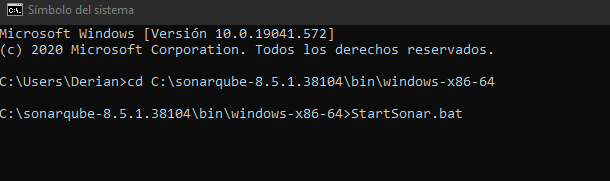
\includegraphics[width=15cm, height=5cm]{img/star.png}  
    \end{center}
    \begin{center}
        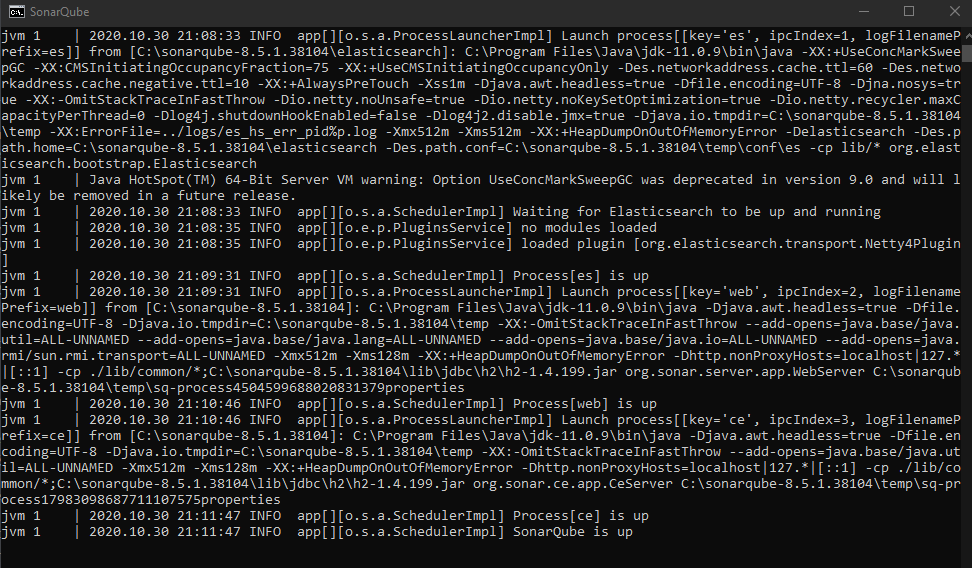
\includegraphics[width=15cm, height=11cm]{img/star2.png}  
    \end{center}

    -Ahora analizaremos el codigo .Ingresamos
     a la direccion de nuestra solucion y ejecutamos el codigo con el nombre
      del proyecto y el nombre de la solucion.
    
     \begin{center}
        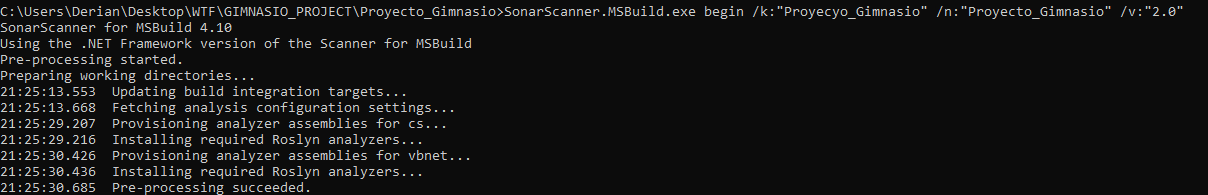
\includegraphics[width=15cm, height=4cm]{img/scan1.png}  
    \end{center}

    -Despues ejecutamos el siguiente codigo para realizar el analisis

    \begin{center}
        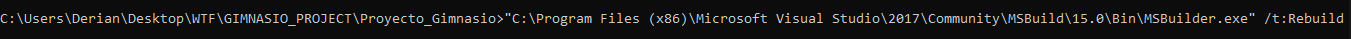
\includegraphics[width=20cm, height=1cm]{img/scan2.png}  
    \end{center}
    -Y por ultimo este codigo para finalizar el analisis.
    \begin{center}
        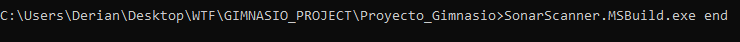
\includegraphics[width=15cm, height=1cm]{img/scan3.png}  
    \end{center}
    -Luego entramos a nuestro localhost de SonarQube.Aqui tenemos el 
    analisis de nuestro proyecto anterior y el que mejoramos.
    \begin{center}
        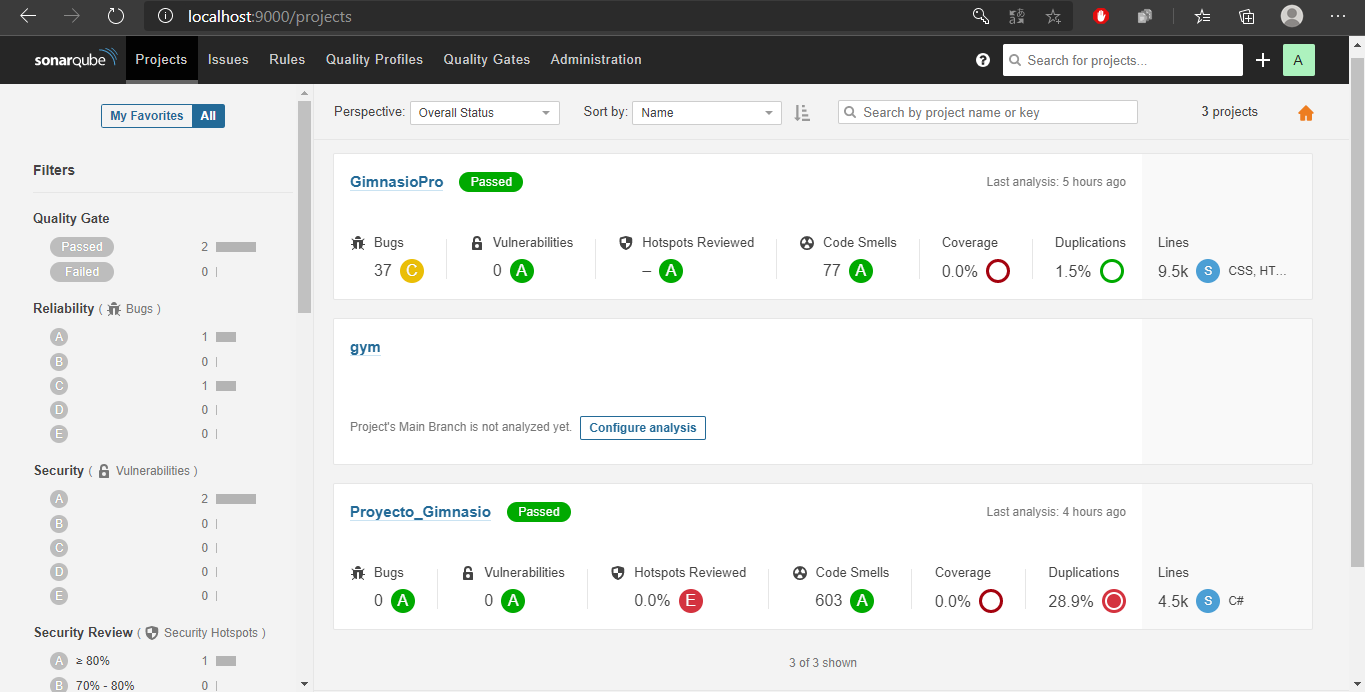
\includegraphics[width=18cm, height=10cm]{img/local1.png}  
    \end{center}
\newpage
-Muestra del analisis de nuestro proyecto anterior:
\begin{center}
    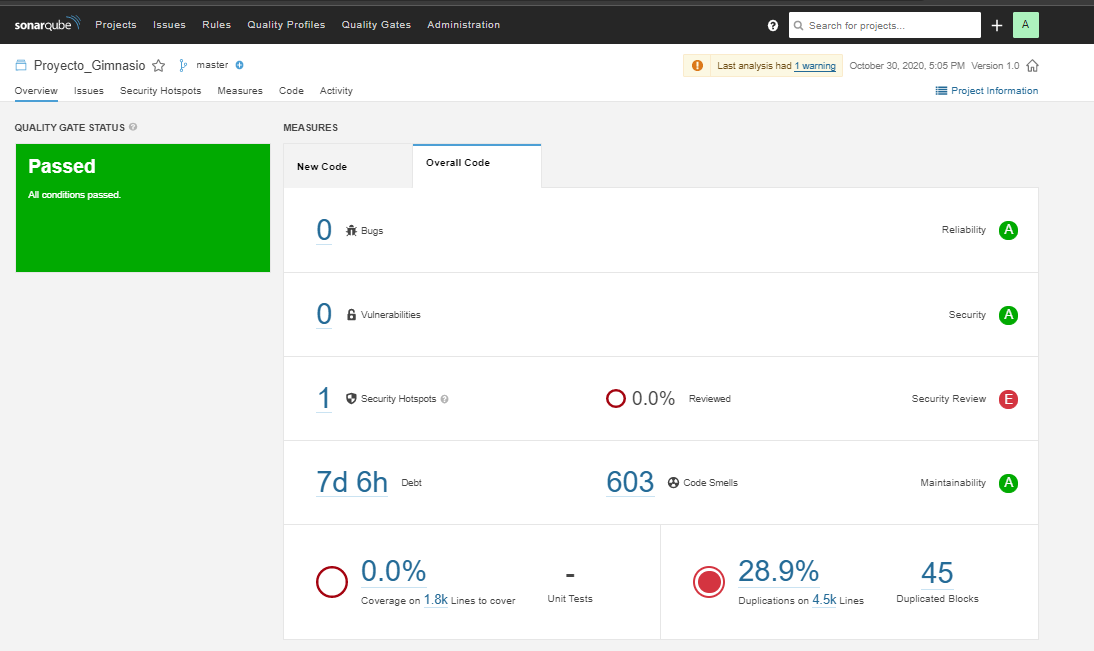
\includegraphics[width=18cm, height=10cm]{img/pro1.png}  
\end{center}
Como vemos tenemos 0 bugs, 0 vulnerabilidades, 1 punto de acceso de seguridad vulnerabilidade,
Una deuda tecnica de  7 dias 6 horas , 603 de codigo que podria ser un problema, casi un 30 porciento de 
duplicidad de codigo en 45 bloques.
\\

\newpage
-Ahora veremos el codigo que realizamos con algunas mejoras como el uso de EntityFramkework

\begin{center}
    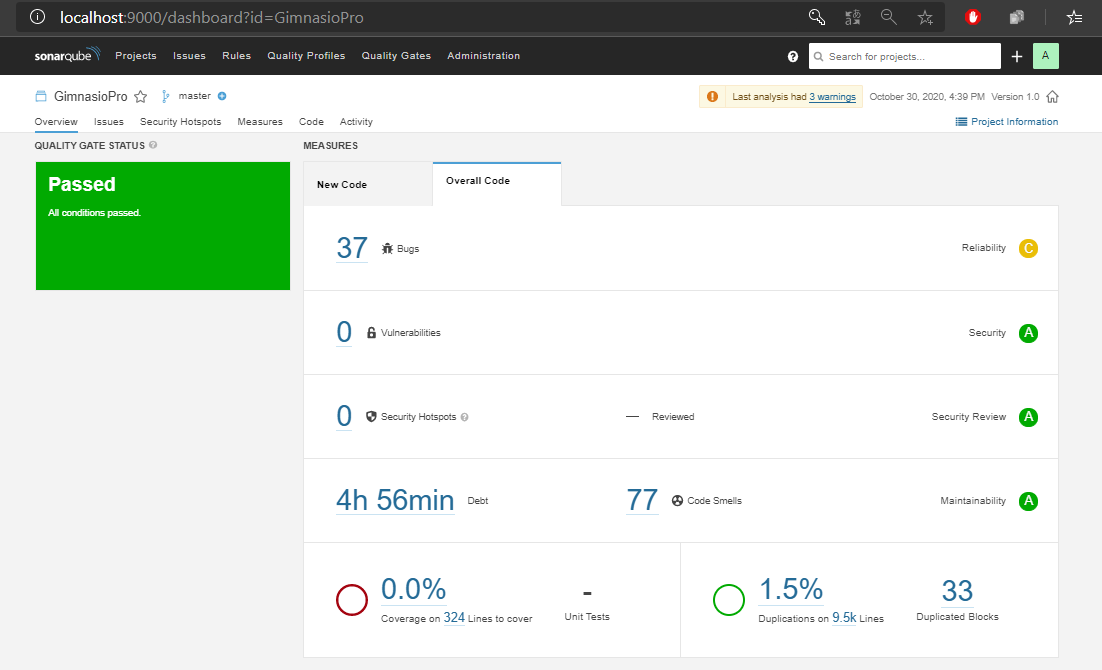
\includegraphics[width=18cm, height=10cm]{img/2scan.png}  
\end{center}

En este caso nuestra solucion tiene 37 bugs. Mas que todos en las vistas del proyecto.
en donde nos pide poner un id y scope a nuestras tablas
\begin{center}
    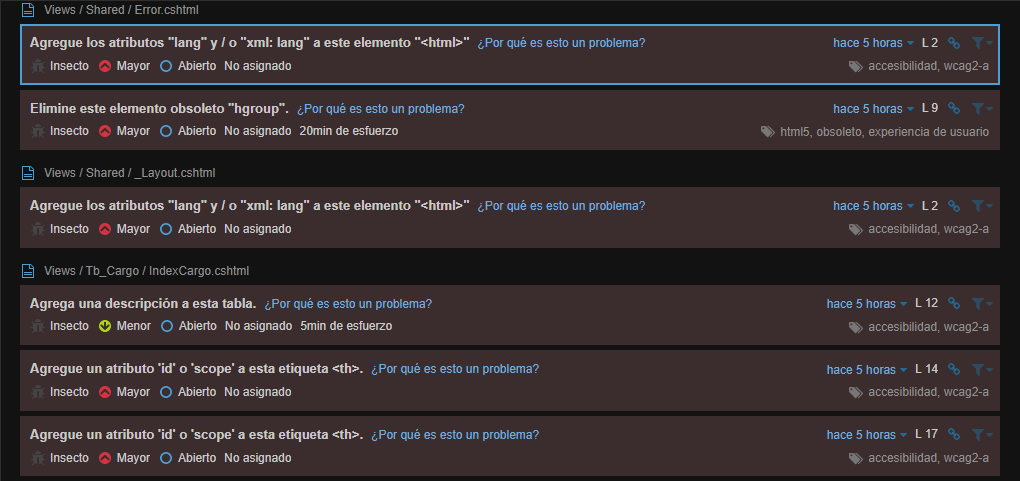
\includegraphics[width=18cm, height=9cm]{img/2scan2.png}  
\end{center}
\newpage
En la parte de seguridad se eliminaron las vulnerabilidades.
\begin{center}
    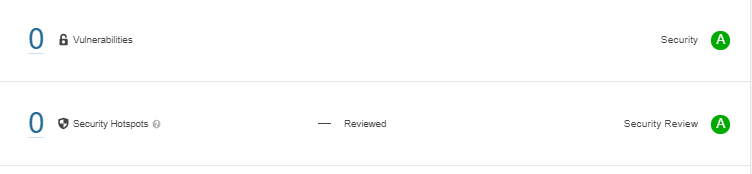
\includegraphics[width=18cm, height=5cm]{img/2scan3.png}  
\end{center}  
\newpage
En lo que se refiere a deuda total tenemos 4h 56 min de deuda.Relacionados a
 41 componentes del proyecto.

\begin{center}
    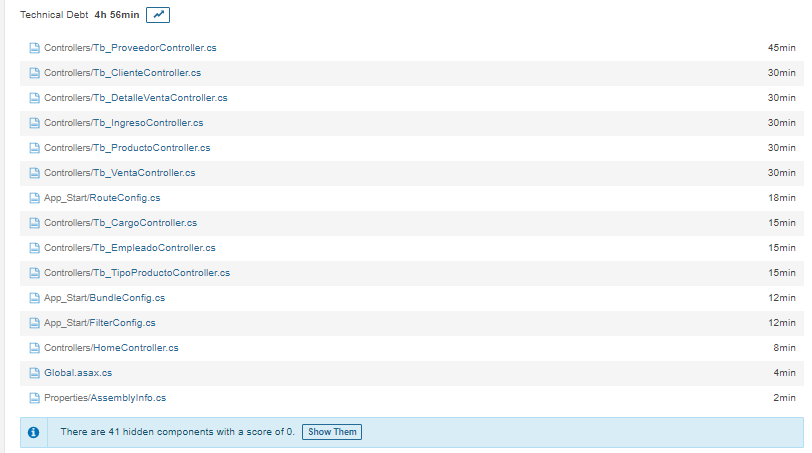
\includegraphics[width=18cm, height=11cm]{img/2scan4.png}  
\end{center}

Se encontro tenemos 324 lineas por cubrir con pruebas unitarias estas
relacionados con14 componentes de nuestro proyecto.
\begin{center}
    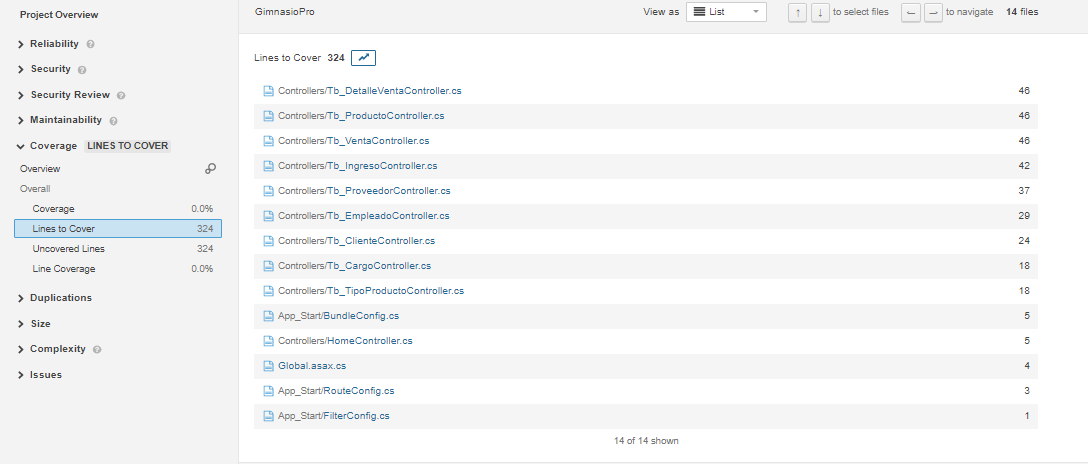
\includegraphics[width=18cm, height=9cm]{img/2scan5.png}  
\end{center}

Tenemos codigo peligro que puede dañar a un futuro el proyecto que tiene que ver 
en el uso innecesarios de codigo y agregar contrucctores de proteccion.
\begin{center}
    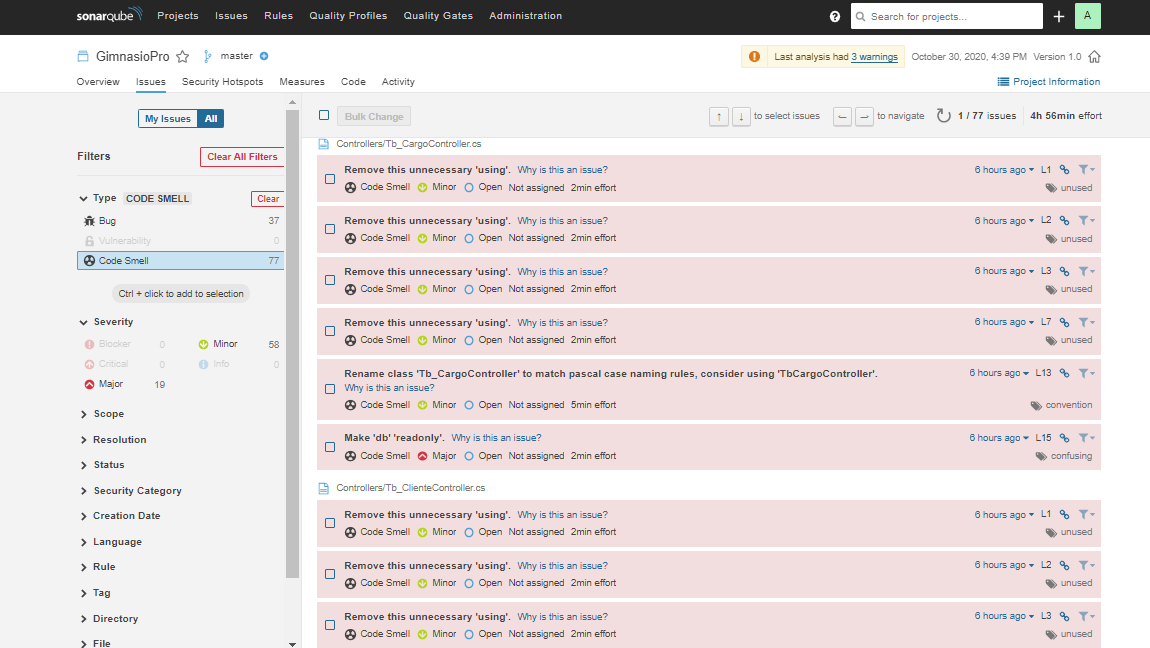
\includegraphics[width=18cm, height=9cm]{img/2scan6.png}  
\end{center}

Encontramos duplicidad de codigo producto de malas practicas al programar,
 pero esta en el rango de aceptacion
 \begin{center}
    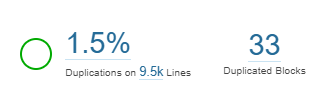
\includegraphics[width=10cm, height=3cm]{img/2scan7.png}  
\end{center}
\newpage
Medidas
\begin{center}
    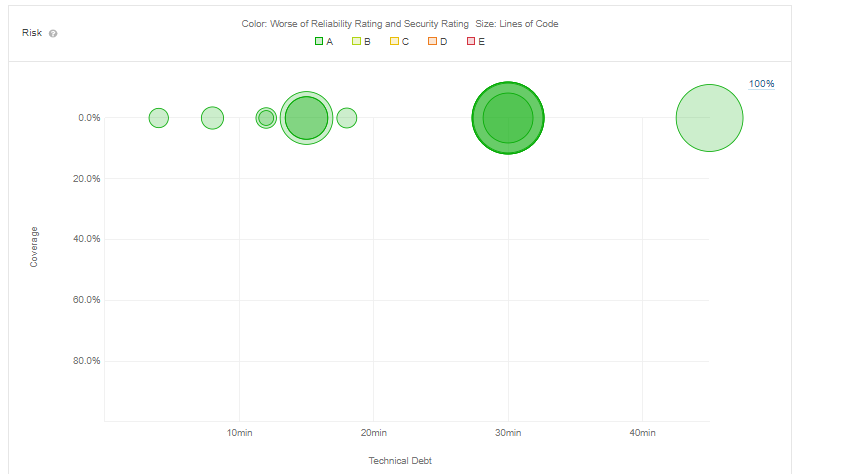
\includegraphics[width=18cm, height=10cm]{img/2scanF.png}  
\end{center}


\section{Cronograma}    
\begin{center}
    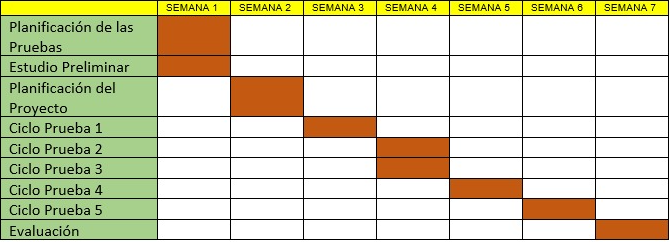
\includegraphics[width=18cm, height=10cm]{img/crono.png}  
\end{center}

\section{ Desarrollo de Solución de Mejora}    
\subsection{Diagrama de Arquitectura de la aplicación}
\begin{center}
    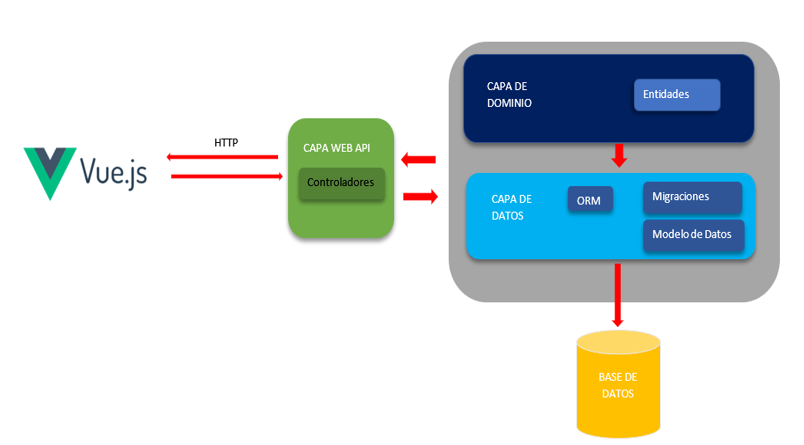
\includegraphics[width=18cm, height=10cm]{img/arqui.png}  
\end{center}
\subsection{Diagrama de Clases de la aplicación}
\begin{center}
    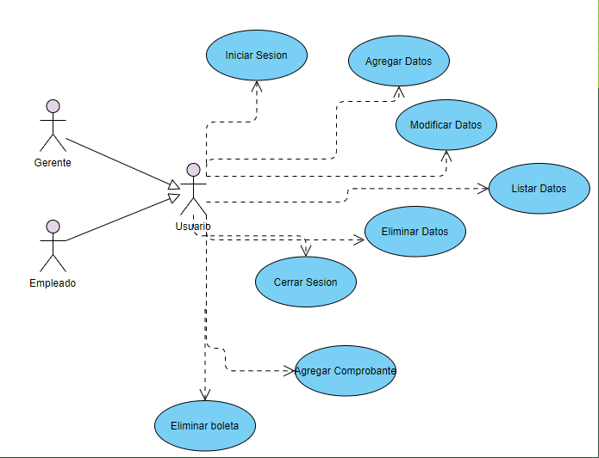
\includegraphics[width=18cm, height=10cm]{img/casos.png}  
\end{center}
\begin{center}
    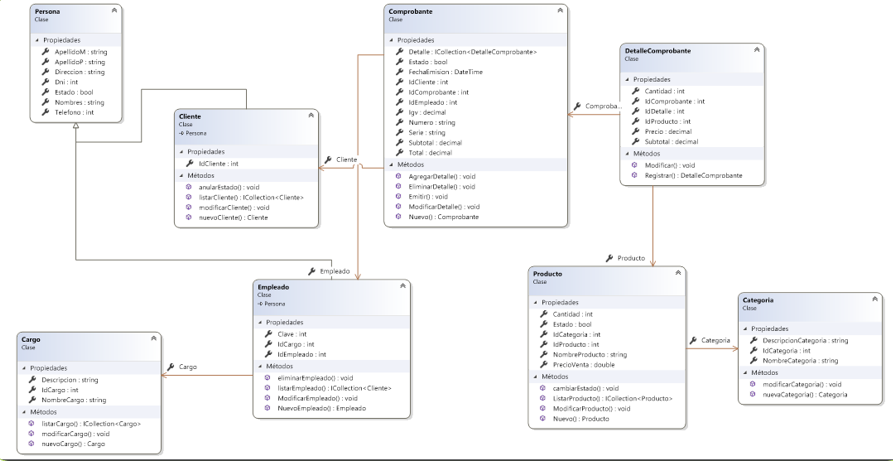
\includegraphics[width=18cm, height=10cm]{img/casos2.png}  
\end{center}
\newpage
\subsection{Metodos de pruebas implementados para coberturar la aplicación}

a) Pruebas Unitarias (cobertura de al menos 70% de codigo)
\begin{center}
    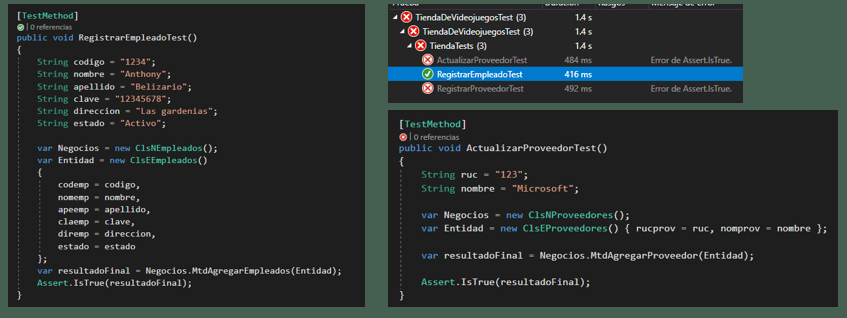
\includegraphics[width=18cm, height=10cm]{img/test1.png}  
\end{center}
\begin{center}
    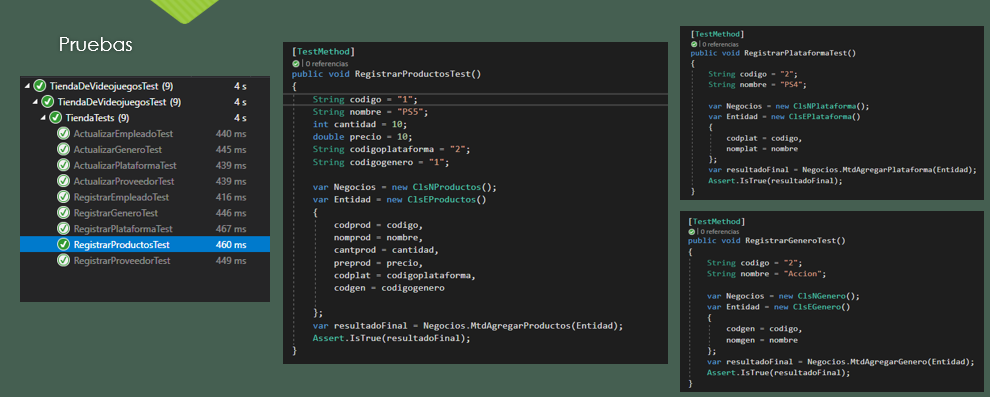
\includegraphics[width=18cm, height=10cm]{img/tes2.png}  
\end{center}
b) Pruebas de aceptación basadas en Desarrollo Guiado por el Comportamiento una por cada caso de uso o historia de usuario, pueden ser de funcionales o APIs
\begin{center}
    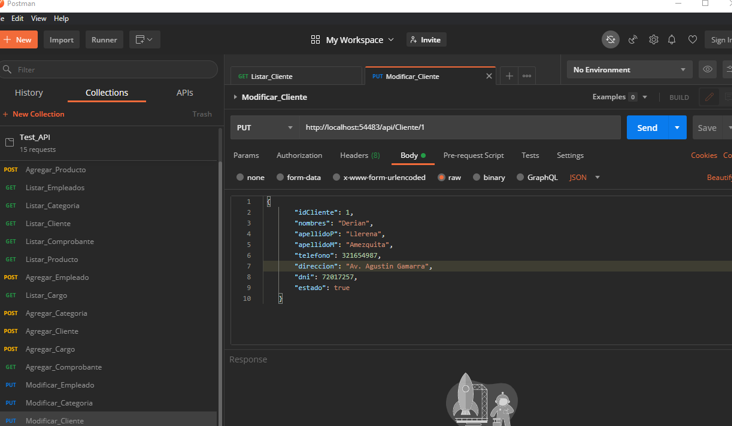
\includegraphics[width=18cm, height=10cm]{img/api1.png}  
\end{center}
\begin{center}
    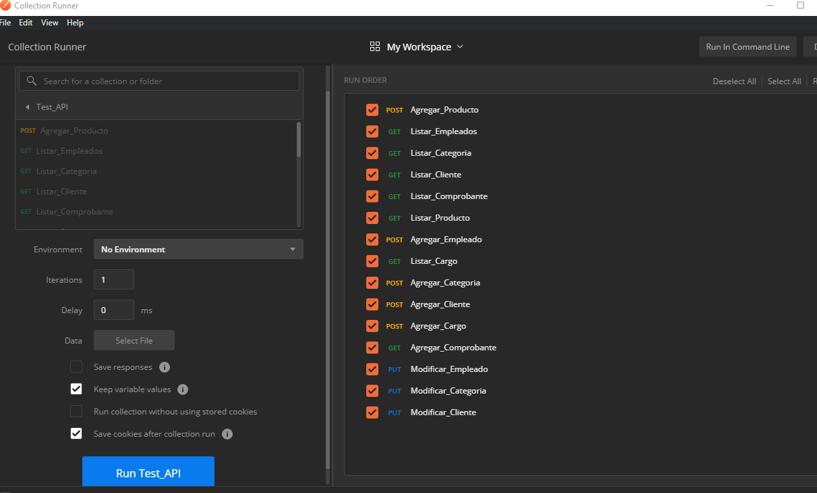
\includegraphics[width=18cm, height=10cm]{img/api2.png}  
\end{center}
\begin{center}
    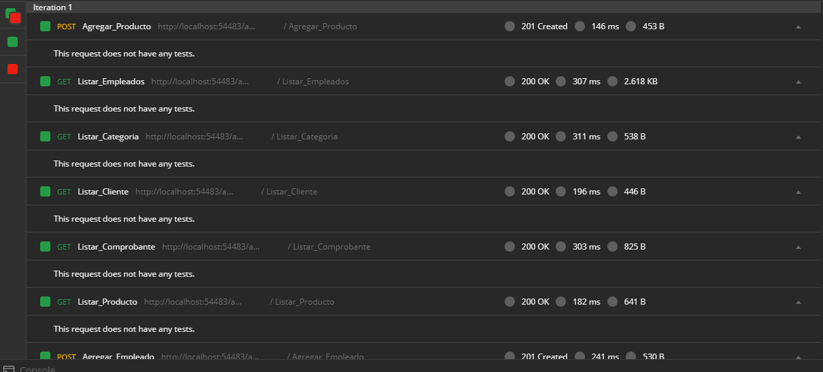
\includegraphics[width=18cm, height=10cm]{img/api3.png}  
\end{center}
\begin{center}
    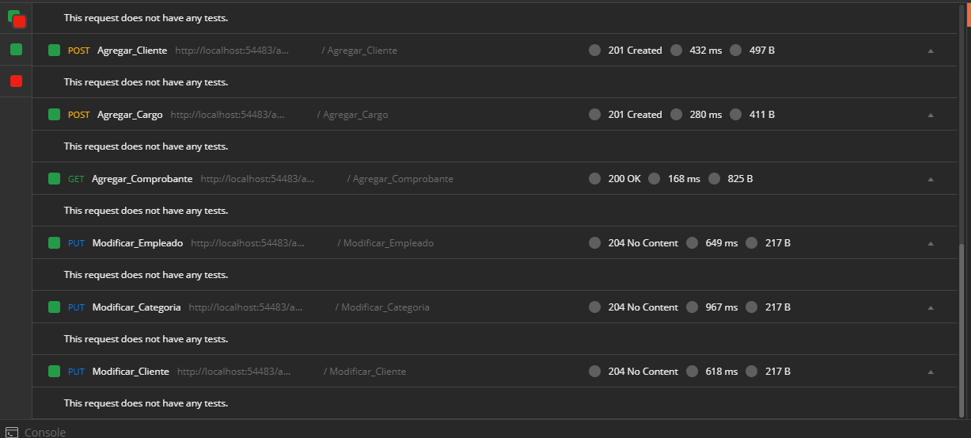
\includegraphics[width=18cm, height=10cm]{img/api4.png}  
\end{center}
\end{document}
